\documentclass[11pt]{article}
\usepackage[utf8]{inputenc}
\usepackage[T1]{fontenc}
\usepackage[french]{babel}
\usepackage{amsmath}
\usepackage[bookmarks={true},bookmarksopen={true}]{hyperref}
\usepackage{graphicx}
\usepackage[a4paper]{geometry}
\usepackage{listings}
\usepackage{amssymb}
\usepackage{amsmath,amsfonts}
	\lstset{frame=tb,
		language=Java,
 		aboveskip=3mm,
  		belowskip=3mm,
  		showstringspaces=false,
  		columns=flexible,
  		basicstyle={\small\ttfamily},
  		numbers=none,
 		numberstyle=\tiny\color{gray},
  		keywordstyle=\color{blue},
  		commentstyle=\color{dkgreen},
  		stringstyle=\color{mauve},
  		breaklines=true,
  		breakatwhitespace=true
  		tabsize=3
	}
\pagestyle{plain}
\setlength{\parindent}{5mm}
\usepackage{amsmath}
\usepackage{color}
\definecolor{dkgreen}{rgb}{0,0.6,0}
\definecolor{gray}{rgb}{0.5,0.5,0.5}
\definecolor{mauve}{rgb}{0.58,0,0.82}



\title{\textbf{Projet LSINF1121 -  Algorithmique et structures de données\\ - \\ Rapport intermédiaire Mission 4} \\ {\large Groupe 26}}
\author{Laurian \bsc{Detiffe} \\(6380-12-00)\and Sundeep \bsc{Dhillon} \\(6401-11-00)\and Alexis \bsc{Macq} \\ (5910-12-00) \and Xavier \bsc{Pérignon} \\ (8025-11-00)\and Thibaut \bsc{Piquard}\\(4634-13-00)\and Thomas \bsc{Wyckmans} \\ (3601-12-00)}
\date{date}
\date{\vspace*{25mm}

\includegraphics[scale=0.75]{logo.jpg}\\
		\vspace*{30mm}
		\begin{center}
		Année académique 2015-2016 \\	
		\end{center}}

\begin{document}
\thispagestyle{empty}

\maketitle
\thispagestyle{empty}
%\tableofcontents
%\setcounter{tocdepth}{3}
%\setcounter{page}{1}
%\newpage

\section*{Questions et réponses}
\begin{enumerate}
\item Citez au moins quatre implémentations différentes d’un dictionnaire (table de
symboles). Précisez, dans chaque cas, quelles sont les propriétés principales
de ces implémentations. Dans quel(s) cas s’avèrent-elles intéressantes ? Quelles
sont les complexités calculatoires de leurs principales méthodes ? (Xavier)\\
\begin{enumerate}
\item \textbf{Recherche séquentielle (liste désordonnée) :}

Une option simple pour la structure de données d'une table de symboles est une liste chaînée de noeuds qui contiennent des clés et des valeurs. Le principe de l'algorithme est qu'il parcourt la liste en comparant la clé de recherche avec la clé de chaque noeud dans la liste. Si les clés concordent, il retourne la valeur associée. Sinon, il retourne $null$. La mise en œuvre d'une liste liée à la recherche séquentielle est trop lente pour qu'elle puisse être utilisée pour résoudre d'énormes problèmes. Cependant, elle est idéale pour les petits problèmes.

\item \textbf{Binary tree search (BST) :}

Un arbre de recherche binaire est un arbre binaire où chaque noeud a une clé (et une valeur associée) et qui satisfait la restriction que la clé dans un noeud quelconque est plus grande que celle de tous les noeuds du sous-arbre gauche de ce noeud et plus petite que celle de tous les nœuds du sous-arbre droit de ce noeud. La mise en oeuvre de cette structure est très facile à implémenter. Cependant, si l'abre ressemble à une liste chaînée, cela risque d'augmenter fortement la complexité. 

\item \textbf{Separate chaining (tableau de listes) :}

Dans la méthode dite de chaînage séparé, chaque bucket est indépendant, et a une sorte de liste des entrées avec le même index. Le temps d'exécution d'une opération d'une table de hachage est le temps de trouver le bucket (qui est constant) plus le temps de l'opération concernant la liste. Dans une bonne table de hachage, chaque bucket a 0 ou 1 entrée, parfois 2 ou 3, mais rarement plus que cela. Par conséquent, les structures sont efficaces dans le temps et l'espace. Cependant, ce procédé hérite également les inconvénients des listes liées. En effet, lors du stockage de petites clés et de valeurs, la surcharge de l'espace du prochain pointeur dans chaque entrée peut être importante. 

\item \textbf{Linear probing (tableaux parallèles) :}

Linear probing est réalisée en utilisant deux valeurs : une étant comme une valeur de départ et une autre étant comme un intervalle entre les valeurs successives en arithmétique modulaire. La seconde valeur, qui est la même pour toutes les clés et connue sous le nom $stepsize$, est ajoutée à plusieurs reprises à la valeur de départ jusqu'à ce qu'un espace libre est trouvé, ou que toute la table soit parcourue.
\begin{center}
$newLocation = (startingValue + stepSize) \% arraySize$
\end{center}
Cet algorithme offre une bonne mise en cache de la mémoire (si $stepsize$ est égal à 1), grâce à la bonne localité de référence.\\
\end{enumerate}
\textbf{Résumé :}
\begin{center}
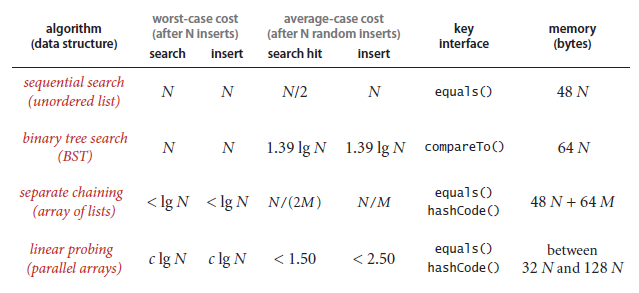
\includegraphics[scale=0.75]{symbol.PNG}
\end{center}
\item Souvenez vous de la question suivante proposée en bilan sur la mission sur les
tris : Étant donné un ensemble $S$ de taille $n$, et un nombre $x$. Décrivez un algorithme
efficace utilisant une HashTable pour trouver s’il existe une paire $(a, b)$
avec $a \in S$, $b \in S$ telle que $a + b = x$. Quelle est la complexité de votre algorithme
? Est-elle meilleure que votre solution qui utilisait un tri ? (Xavier)\\

Concernant le bilan sur la mission sur les tris, la solution était de faire un tri efficace de l'ensemble $S$ (par exemple Quicksort) et ensuite de tester l'addition du premier élément $a$ avec le dernier élément $b$. Si le résultat de cette addition était inférieur à $x$, alors on testait l'addition de $(a+1)$ avec $b$, et ainsi de suite. Sinon si le résultat de l'addition était supérieur à $x$, alors on testait l'addition de $a$ avec $(b-1)$, et ainsi de suite.\\\\
Pour résoudre le même problème avec une HashTable, on pourrait penser à insérer tous les éléments de l'ensemble $S$ dans une HashSet. Cette classe implémente l'interface Set, en utilisant une HashTable. HashSet est implémenté comme une HashMap, dont les clés sont les éléments du HashSet et les valeurs sont toutes une même valeur présente. Cette implémentation offre des performances constantes pour les opérations \textit{add(T t)}, \textit{remove(T t)}, \textit{contains(T t)} et \textit{size()}. Il suffira donc de vérifier si pour chaque élément $a$ de l'ensemble $S$, il existe $b$ dans la HashSet tel que $b = x - a$. La complexité de cet algorithme est donc de $O(1)$ + $O(n)$ (parcours des éléments de $S$). Ce qui est plus rapide que l'algorithme de la mission sur les tris.\\

\item Démontrez que $(a + b)\%M$ est équivalent à $((a\%M) + b)\%M$. En quoi cette 
propriété peut être utile pour construire une fonction de hachage sur les String.
Expliquez comment Java calcule une fonction de hachage sur les String ? Quelle
est la complexité pour calculer 1 fois et N fois le hashcode d’un String. (Xavier)\\

Prenons G = $(a + b)\%M$ et D = $((a\%M) + b)\%M$.\\ 
On doit démontrer que G = D.\\
Nous pouvons écrire :
\begin{center}
a = M * Q1 + R1 where 0 $\le$ R1 < M où Q1 est un entier. a mod M = R1\\
b = M * Q2 + R2 where 0 $\le$ R2 < M où Q2 est un entier. b mod M = R2\\
(a + b) = M * (Q1 + Q2) + R1+R2 \\
G = (a + b) mod M\\
G = (M * (Q1 + Q2) + R1+ R2) mod M\\
\end{center} 
On peut supprimer les multiples de M lorsqu'on prend mod M,
\begin{center}
G = (R1 + R2) mod M\\
D = (a mod M + b) mod M\\
D = (R1 + R2) mod M\\
\end{center}
Et donc, 
\begin{center}
G = D = (R1 + R2) mod M\\
\end{center}
\vspace{1\baselineskip}
Cette propriété est utile pour construire une fonction de hashage sur les String car il n'est pas nécessaire de calculer le modulo de chaque valeur des caractères du String. En effet, il suffira de calculer la somme de la valeur des caractères et utiliser une seule fois le modulo à la fin.\\\\
La fonction de hashage pour un String est implémentée comme suit :
\begin{center}
$s[0]*31^{(n-1)} + s[1]*31^{(n-2)} + ... + s[n-1]$
\end{center}
Dans cette fonction, le String $s$ a $n$ caractères. Elle calcule la somme des valeurs de chaque caractère, chacun multiplié par $31^{r}$ avec $r$ étant l'emplacement inversé du caractère dans le String. La complexité du calcul de hashcode d'un String est de $O(n)$ puisqu'il faut parcourir tous les caractères du String. Mais une fois ce calcul fait, il n'est plus nécessaire de recalculer le hashcode de ce String.\\

\item
\item 
\item 
\item
\item 
\item 
\item
\item 


\end{enumerate}
\end{document}
